\section{异步推理收益的实验验证}\label{sec:async-exp}

\subsection{实验目的与论证逻辑}\label{sec:async-exp-purpose}

4.2 节给出的分段模型说明，异步推理的理想 FPS--异步推理触发阈值曲线应当具有清晰的临界点：
临界点之前，异步推理触发阈值越大，触发越早，stall 越短，有效 FPS 随之上升；
越过临界点之后，新动作 chunk 能在旧队列耗尽前返回，系统应饱和到目标 30 FPS。
因此，本实验的核心目的不是证明``异步推理触发阈值越大越好''，
而是在树莓派 5 单机部署条件下寻找这个实际临界点，
并解释为什么实测 episode 平均 FPS 没有完全达到理论上的 30 FPS。

评价逻辑分为两层。第一层是动作可完成性：
若某个异步推理触发阈值导致抓取轨迹明显漂移或任务成功率下降，则即使帧率较高也不可采用。
第二层才是流水线收益：在动作质量合格的配置中比较有效 FPS、
stall 比例和推理耗时分布。

需要特别说明的是，在当前代码实现中，触发条件是动作队列剩余比例不高于 hold，
因此异步推理触发阈值越大表示越早触发推理。
这与直觉中``阈值越小越早''的说法相反，后文分析均按代码语义展开。

\subsection{实验配置与记录方式}\label{sec:async-exp-design}

实验采用异步推理触发阈值单变量扫描。同步 baseline 复用实验 04 中无 tracing 的
A 组记录，异步模式固定 chunk\_size $N=100$、目标频率 $F=30$ FPS，
在同一 ACT 模型与同一 pick 任务下扫描异步推理触发阈值0.10--0.60，
其中 0.60 作为偏早触发的参考点。
每个异步推理触发阈值当前采集 1 个 60 s episode，动作质量由操作者现场观察记录；
CSV 中 success=-1 表示本轮尚未写入机器可读成功/失败标签。

\begin{table}[htbp]
  \centering
  \caption{异步推理触发阈值扫描实验配置}
  \label{tab:async-exp-config}
  \begin{tabularx}{\textwidth}{@{}p{0.22\textwidth}Xp{0.24\textwidth}@{}}
  \toprule
  维度 & 取值 & 备注 \\
  \midrule
  调度模式 & 同步 / 异步 & 同步作为 baseline \\
  chunk\_size $N$ & 100 & 同第三章设置 \\
  目标 FPS $F$ & 30 & environment\_dt = 33.3 ms \\
  异步推理触发阈值 & 0.10, 0.20, 0.25, 0.30, 0.35, 0.40, 0.50, 0.60 & 异步调度参数 \\
  episode 时长 & 60 s & 每个阈值 1 次 \\
  同步 baseline & 16.13 FPS & 实验 04 A 组无 tracing \\
  \bottomrule
  \end{tabularx}
\end{table}

数据文件与脚本统一放在
lerobot/analysis/08\_async\_inference\_hold\_sweep/：
client 端输出逐 episode 的统计文件，记录动作执行帧数、stall 帧数、
过期帧数、must\_go 触发次数和帧率等；server 端输出逐次推理的耗时文件；
此外新增 stall 事件记录，追踪每次队列耗尽到恢复的起止时间和持续帧数。
离线分析时由脚本将 client 与 server 的记录按时间戳对齐合并后绘图。

\subsection{打点与对齐方法}\label{sec:async-exp-metrics}

client 端记录的核心指标包括：执行帧数、stall 帧数、过期帧数、
must\_go 触发次数、帧率统计以及 CPU 温度与频率。其中有效 FPS 定义为：
\begin{equation}
  F_{\text{eff}} = \frac{\mathrm{action\_frames}}{\mathrm{episode\_total\_s}}.
\end{equation}
该指标只统计真正执行了 action 的帧，能剔除 stall 停顿对名义循环频率的影响。

本次采集新增了 stall 事件追踪：每当控制循环发现动作队列已空时，
记录当时的帧号和episode内时间作为 stall 起始点；
当队列重新有数据可执行时记录 stall 结束点，从而得到每段连续停顿的持续时间。
该信息用于判断 stall 是集中在启动阶段还是均匀分布在整个 episode。

server 端在每次推理前后分别记录时间戳，输出该次推理的耗时。
本轮采集期间 server 进程持续运行，没有随 client 侧 episode 切分而重启，
导致 server 日志中的 episode 编号与 client 不对齐；
因此离线合并时通过检测 server 日志中帧号回跳的位置来切分各 episode 的推理记录，
恢复与 client 端的对应关系。

\subsection{实验结果}\label{sec:async-exp-results}

图~\ref{fig:async-hold-fps} 给出有效 FPS 随异步推理触发阈值变化的折线。
同步 baseline 为 16.13 FPS；异步各阈值的有效 FPS 位于
19.96--27.42 FPS 之间，相对同步提升 23.8\%--70.0\%。
图中将同步 baseline 放在触发阈值为0的位置作为参照点，
并对 baseline--0.30 区间做线性拟合。
需要强调的是，4.2 节的理想模型是直接由执行时间、计算时间和 stall 时间相加得到的；
这里的线性拟合只对应临界点之前、一定存在 stall 的前段区间，
用于描述实测点近似线性上升的趋势。
从 0.10 到 0.30，FPS 随异步推理触发阈值增大快速上升；
0.30 和 0.35 已经接近满帧状态，episode 平均 FPS 约为 27 FPS。
理想模型中该区间理论上应达到 30 FPS 的满帧水平，实测仍有约 2--3 FPS 缺口，
主要来自 episode 启动阶段的必然空队列等待，以及树莓派 5 上
控制端进程、推理服务进程、相机线程和串口通信共享 CPU
造成的调度抖动。

\begin{figure}[htbp]
  \centering
  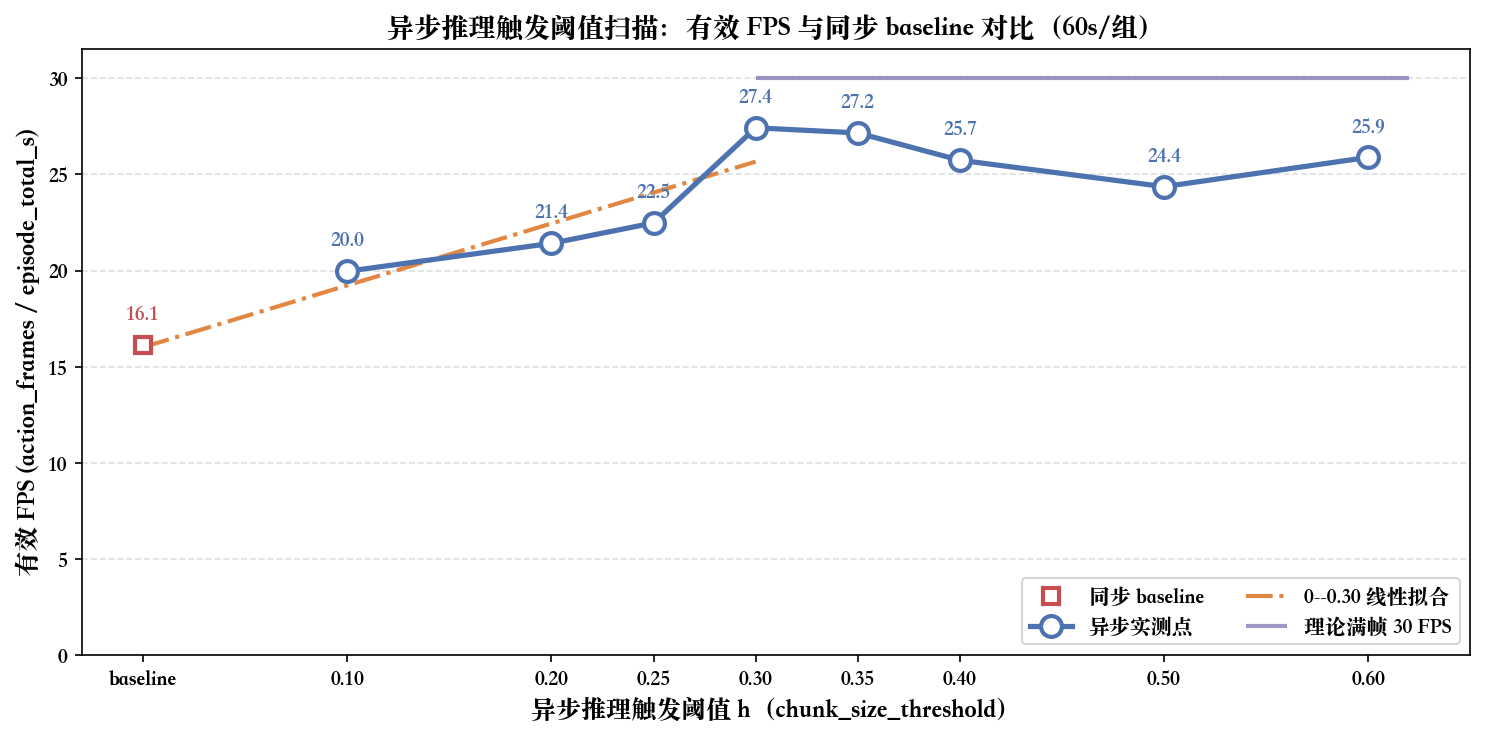
\includegraphics[width=0.92\textwidth]{4_优化/images/chart1_fps_vs_sync.png}
  \caption{异步推理触发阈值扫描}
  \label{fig:async-hold-fps}
\end{figure}

对图~\ref{fig:async-hold-fps} 的理解可以分为三个部分。横轴表示异步推理触发阈值，
阈值越大表示越早请求下一段动作；纵轴表示实际执行动作的有效 FPS。
左侧同步 baseline 用来说明未引入异步推理时的基准水平，右侧各点则表示不同阈值下的异步运行结果。
从曲线趋势看，阈值从 0.10 增大到 0.30 时，有效 FPS 明显上升，
说明提前触发推理能够减少动作队列耗尽造成的 stall。
当阈值继续增大后，曲线没有继续明显上升，而是在接近满帧的位置附近波动，
这说明系统已经接近异步流水线的临界区间；
此时继续提前触发推理不一定带来更高帧率，反而可能增加观测过期和动作块错位风险。
因此，该图的重点不是寻找最大的阈值，而是识别 FPS 提升趋于饱和前后的临界范围。

表~\ref{tab:async-hold-results} 汇总了核心指标。

\begin{table}[htbp]
  \centering
  \caption{异步推理触发阈值扫描核心结果（每个阈值 1 个 60 s episode）}
  \label{tab:async-hold-results}
  \begin{tabular}{cccccc}
  \toprule
  异步推理触发阈值 & 动作质量 & 有效 FPS & 相对提升 & stall\% & expire\% \\
  \midrule
  0.10 & 很好     & 19.96 & 23.8\% & 31.78 & 32.05 \\
  0.20 & 很好     & 21.41 & 32.8\% & 26.53 & 41.27 \\
  0.25 & 很好     & 22.48 & 39.4\% & 23.18 & 39.07 \\
  0.30 & 很好     & 27.42 & 70.0\% &  5.35 & 49.45 \\
  0.35 & 一般     & 27.16 & 68.4\% &  5.56 & 49.25 \\
  0.40 & 一般     & 25.74 & 59.6\% &  9.65 & 49.33 \\
  0.50 & 一般     & 24.36 & 51.1\% & 13.23 & 49.17 \\
  0.60 & 较差     & 25.89 & 60.5\% &  9.33 & 49.36 \\
  \bottomrule
  \end{tabular}
\end{table}

从 stall 事件的时序分布来看，不同异步推理触发阈值下的 stall 形态差异非常显著。
异步推理触发阈值为0.30的 60 s episode 中仅出现 2 次 stall：第一次在 episode 启动时
持续约 2 s（61 帧），第二次在 frame 162 附近持续约 1 s（32 帧），
之后稳态阶段再无 stall。这说明 0.30 已经非常接近实际临界点：
启动瞬态结束后，新 chunk 基本能在队列耗尽前返回，流水线可以自持运转。

而异步推理触发阈值为0.25时的 stall 事件则呈现周期性：几乎每隔 4--5 s 就出现一次
持续约 1 s 的 stall，全 episode 共 13 次。这说明 0.25 的触发已经偏晚，
server 的推理节奏跟不上队列消耗，形成``队列耗尽$\to$must\_go 兜底$\to$
新 chunk 到达$\to$短暂恢复$\to$再次耗尽''的周期性 stall 模式。

异步推理触发阈值为0.50时的 stall 虽然单次持续时间更短（多为 3--10 帧，约 0.1--0.3 s），
但发生频率很高，全 episode 出现 28 次。
这类短 stall 不再是理论模型中的``触发太晚''，
而更像接近满帧时的实现误差：client 频繁采观测、server 端推理、
gRPC 收发、相机后台线程和舵机串口通信都在 4 个 ARM 核心上竞争资源，
使得本应覆盖住的返回时延偶尔越过队列余量。

图~\ref{fig:async-hold-breakdown} 给出执行帧、过期帧和 stall 帧的组成。
随着异步推理触发阈值增大，过期帧比例从 32.05\% 上升至 49.45\%，这与
$T_{\text{infer}}F/N \approx 1.5\times30/100=45\%$ 处于同一量级；
stall 冻结最新已执行动作步号会保护一部分未来帧不被判定为过期，
因此异步推理触发阈值为0.10和0.20时的实测expire\%低于直接代入的理论值。

\begin{figure}[htbp]
  \centering
  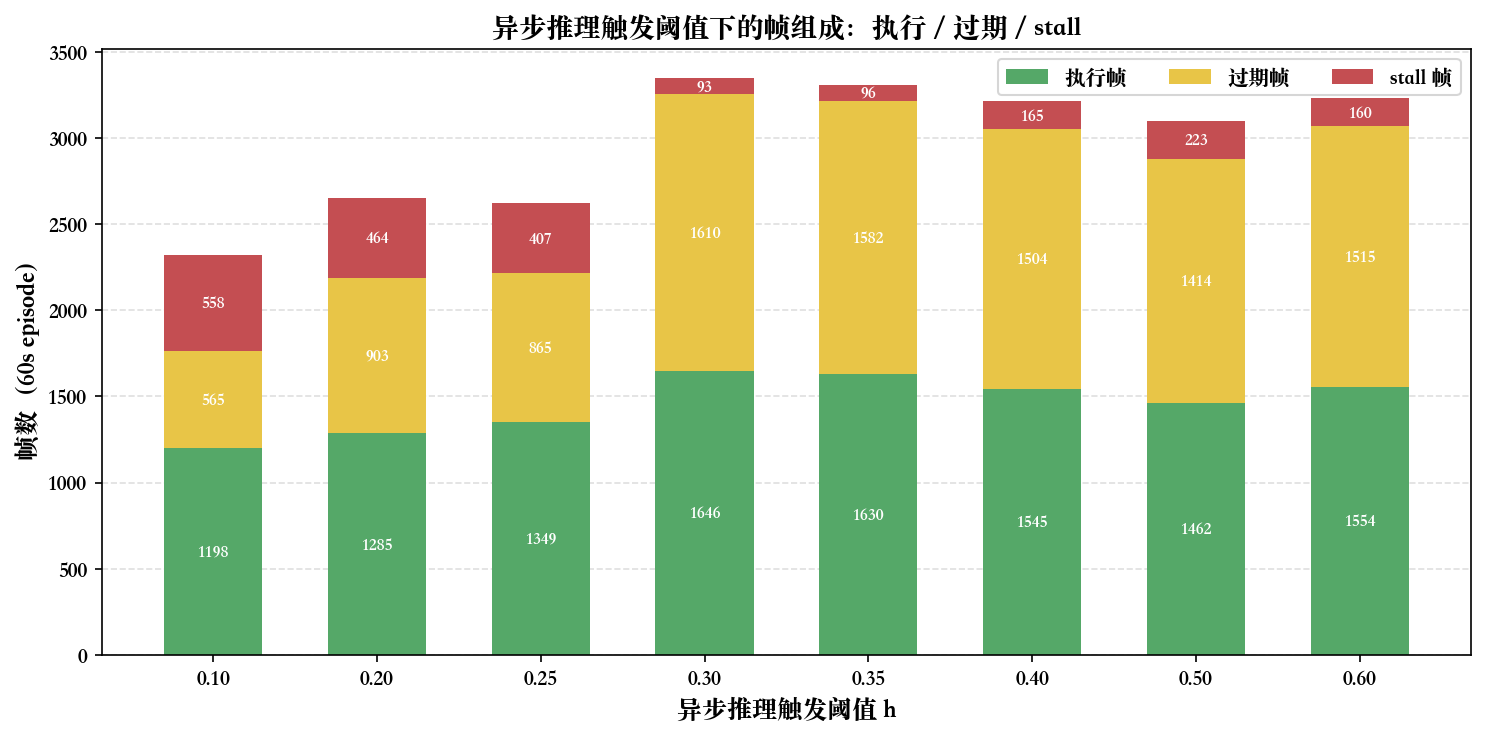
\includegraphics[width=0.92\textwidth]{4_优化/images/chart3_frame_breakdown.png}
  \caption{异步推理中的执行帧、过期帧与 stall 帧组成}
  \label{fig:async-hold-breakdown}
\end{figure}

\subsection{结果讨论}\label{sec:async-exp-discussion}

实验结果与 4.2 节的分段模型基本一致。
异步推理触发阈值为0.10、0.20和0.25时仍处在临界点之前，
stall 呈周期性出现，FPS 随异步推理触发阈值增大而上升；
异步推理触发阈值达到0.30后周期性stall基本消失，
说明实际临界点位于 0.25--0.30 附近。
按理想模型，越过该点后稳态 FPS 应饱和到 30 FPS。
实测 0.30 和 0.35 的 episode 平均 FPS 只有约 27 FPS，
并不表示理论曲线在临界点后下降，
而是因为 60 s episode 中仍包含启动空队列等待，
并且树莓派 5 单机部署下推理进程、控制进程和 I/O 线程存在 CPU 资源争抢，
使有效返回时延产生抖动。

从动作质量的角度观察，异步推理触发阈值在0.10至0.30范围内时操作者均评为``很好''，
0.35、0.40 和 0.50 为``一般''，0.60 动作明显变差评为``较差''。
这说明在本平台参数下，动作质量对异步推理触发阈值的敏感度低于有效 FPS 和 stall 比例：
即使异步推理触发阈值为0.10时的stall高达31.78\%，有效 FPS 仅为 19.96，
temporal ensemble 仍然能在多数时刻维持轨迹连贯性。
异步推理触发阈值继续增大后，虽然理论 FPS 已经接近满帧，
但更频繁地发送观测、融合动作和触发短 stall 会增加控制抖动，
因此动作质量反而开始下降。
这一现象也与近期关于异步动作分块的讨论一致：
异步推理虽然可以提高响应频率，但若返回的动作块与当前观测或已执行状态发生错位，
仍可能引入 chunk 内部不一致和轨迹抖动\cite{remac}。
因此在实际部署中，可以优先依据有效 FPS 和 stall 比例来选择异步推理触发阈值，
不必过度担心动作质量——只要 stall 不要极端严重（如 0.10 的 31\%），
动作质量仍可保持在可接受范围内。

综合有效 FPS、stall 比例、must\_go 触发次数和动作质量四个维度，
在当前树莓派 5 + ACT 模型的单轮扫描实验中，异步推理触发阈值取 0.30 时表现最佳。
该配置下有效 FPS 达到 27.42，相对同步 baseline 提升 70.0\%，
stall 比例仅 5.35\%，且 must\_go 仅触发 2 次（集中在启动阶段），
稳态阶段几乎无 stall，动作质量被操作者评为``很好''。
异步推理触发阈值为0.35时的 FPS 和 stall 比例与 0.30 几乎相同，但动作质量降为``一般''，
因此不推荐作为默认值。

该结论也为后续优化提供方向。若进一步通过 ONNX Runtime、量化或算子优化
把有效返回时延 $T_{\text{rt}}$ 降至 1.0 s 左右，
则临界异步推理触发阈值将下降到
$1.0\times30/100=0.30$，且 $T_{\text{rt}}F=30 < N/2=50$，
0.30 将从临界点变成有明显余量的稳定配置。
若希望更晚触发、进一步减少过期帧和 temporal ensemble 冲突，
则需要把 $T_{\text{rt}}$ 继续压低；例如异步推理触发阈值为0.20时若要进入无stall区，
有效返回时延需接近 $0.20\times100/30\approx0.67$ s。
